Throughout this chapter, we fix a category $\mathcal{C}$.
\begin{definition}[Weighted Type Graph~\cite{endrullis2024generalized_arxiv_v2}]
    \label{wf:def:weighted_type_graph}
    A \textbf{weighted type graph} is a tuple~\(\mathcal{T} = (T, \mathbb{E}, \mathcal{S}, w)\) where
    \begin{itemize} 
        \item \(T\) is an object of $\mathcal{C}$, called \textbf{type graph},
        \item \(\mathbb{E}\) is a set of morphisms in $\mathcal{C}$ with codomain $T$; the elements of \(\mathbb{E}\) are called \textbf{morphism-rulers};
        \item \(\mathcal{S}=(S, \oplus, \odot, 0, 1)\) is a commutative semiring,
        \item \(w : \mathbb{E} \to S \setminus \{0\}\) is a weight function such that for all $e \in \mathbb{E}, w(e) \geq 1$
    \end{itemize}
    % The weighted type graph \(\mathcal{T}\) is \textbf{finitary} if for every \( (e :X \to T) \in \mathbb{E}\) and every object \(G\), \(\operatorname{Hom}(X, G)\) and \(\operatorname{Hom}(G, T)\) are finite sets.
    such that for every \( (e :X \to T) \in \mathbb{E}\) and every object \(G\), \(\operatorname{Hom}(X, G)\) and \(\operatorname{Hom}(G, T)\) are finite sets.
\end{definition}

\begin{example}
    \label{wf:example:weighted_type_graph}
     In \textbf{Graph}, a weighted type graph 
     whose $\operatorname{dom}(\mathbb{E})$ consists of graphs with two vertices and one labeled edge between them
     can be visualized as a graph with weighted labels and weights given as superscripts. For example, the finitary weighted type graph $\mathcal{T} = (T, \mathbb{E}, \mathcal{S}, w)$ with $\mathcal{S}$ as the natural arithmetic semiring $(\mathbb{N}, +_\mathbb{N}, *_\mathbb{N}, 0_\mathbb{N}, 1_\mathbb{N}, <_\mathbb{N},\leq_\mathbb{N})$ defined in~\autoref{def:weight_of_an_object_relative_to_a_type_graph},
     $T$ as the graph illustrated below (without superscripts), $\mathbb{E}=\{e_{11a},e_{12a},e_{21a},e_{11b}\}$ as the set of morphism-rulers where 
     $e_{uvl}$, for all edge from $u$ to $v$ labeled by $l$, has domain 
     \tikz[baseline=-0.5ex]{
        \node[draw,circle] (x) at (0,0) {};
        \node[draw,circle] (y) at (1,0) {};
        \draw[->] (x) -- (y) node[midway, above] {$l$};
    } and image 
    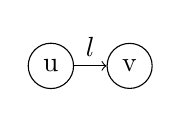
\begin{tikzpicture}[baseline=-2mm]
        \node[draw, circle] (x) at (0,0) {$\mathrm{u}$};
        \node[draw, circle] (y) at (1,0) {$\mathrm{v}$};
        \draw[->]  (x) -- (y) node [midway,above] {$l$};
    \end{tikzpicture} in the graph $T$,
    and $w(e) = 1_\mathbb{N}$ for all $e \in \mathbb{E}$, is visualized in~\autoref{fig:weighted_type_graph_instance}. To improve readability, we omit the subscripts.
    \begin{figure}[H]
        \centering
        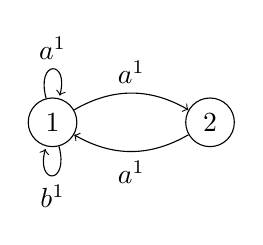
\begin{tikzpicture}
            \graphbox{}{0mm}{0mm}{32mm}{28mm}{-10mm}{-14mm}{
                \node[draw,circle] (1) at (0,0) {1};
                \node[draw,circle] (2) at (2,0) {2};
                \draw[->] (1) edge[loop above] node[midway, above] {$a^{1}$} (1) ;
                \draw[->] (1) edge[loop below] node[midway, below] {$b^{1}$} (1) ;
                \draw[->] (1) edge[bend left] node[midway, above] {$a^{1}$}  (2)  ;
                \draw[->] (2) edge[bend left] node[midway, below] {$a^{1}$} (1)   ;
            }
        \end{tikzpicture}
        \caption{Weighted type graph instance}
        \label{fig:weighted_type_graph_instance}
    \end{figure}
\end{example}